\documentclass[12pt]{article}
\usepackage[english]{babel}
\usepackage[margin=0.5in]{geometry}
\usepackage{hyperref}
\usepackage{amsmath,textcomp,blindtext,xcolor,multicol,color,comment,wrapfig,graphicx,amsthm}
\newtheoremstyle{colored}
  {\topsep}   % Space above
  {\topsep}   % Space below
  {}          % Body font
  {}          % Indent amount
  {\bfseries\color{red}} % Theorem head font - red color for 'def'
  {}          % Punctuation after theorem head
  {.5em}      % Space after theorem head
  {\thmnote{ \textbf{\color{red}#3}}} % Theorem head spec

\newtheoremstyle{subcolored}
  {\topsep}   % Space above
  {\topsep}   % Space below
  {}          % Body font
  {}          % Indent amount
  {\bfseries\color{blue}} % Theorem head font - blue color for 'subdef'
  {}          % Punctuation after theorem head
  {.5em}      % Space after theorem head
  {\thmnote{ \textbf{\color{blue}#3}}} % Theorem head spec
  
\theoremstyle{colored}
\newtheorem*{defn}{}

\theoremstyle{subcolored}
\newtheorem*{subdefn}{}

\usepackage{fancyhdr}
\usepackage{hyperref} % For hyperlinks

% Define the URL for the footer
\newcommand{\myURL}{https://mohammedbilalns.github.io/Math-Demystified/}

% Set up fancy headers and footers
\pagestyle{fancy}
\fancyhf{} % Clear header and footer
\rfoot{\href{\myURL}{\myURL}} % Set the right part of the footer as a hyperlink


\begin{document}
\begin{center}
  {\LARGE \textbf{Triganometric Functions}} \\
  
\end{center}
\begin{multicols}{2}

\begin{defn}[Angle:]The rotation of a ray from one position to
another along the circumference of a circle is
known as an angle. The initial position of the
ray is called initial side and the final position of
the ray is called terminal side.\\
\begin{center}
  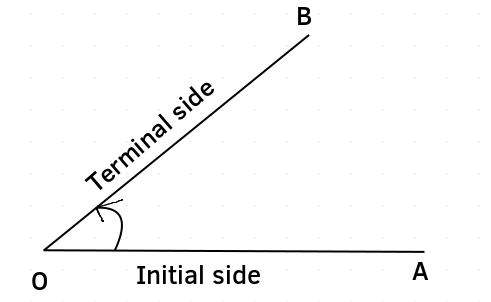
\includegraphics[scale=0.25]{ff.png}
\end{center}

\end{defn}


\begin{subdefn}[Positive Angle:]
  If the rotation of a ray from
one position to another is in anti-clockwise,
then the angle is known as positive angle.\\
\end{subdefn} 

\begin{subdefn}[Negative Angle:]
  : If the rotation of a ray from
one position to another is in anti-clockwise,
then the angle is known as positive angle.

  
\end{subdefn}
\begin{center}
  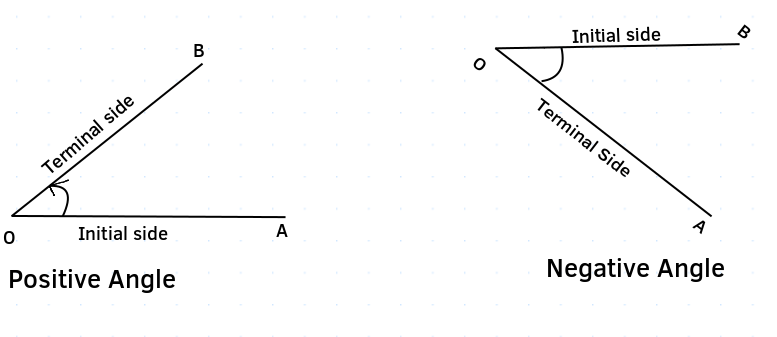
\includegraphics[scale=0.25]{2.png}
\end{center}



    \begin{defn}[Degree Measure:]
      If a rotation from the initial side to terminal side is $(\frac{1}{360})^{th}$ of  
a revolution, the angle is said to have a measure of one degree, written as $1°$. A degree is
divided into 60 minutes, and a minute is divided into 60 seconds . One sixtieth of a degree is
called a minute, written as $1'$, and one sixtieth of a minute is called a second, written as $1"$.
Thus,
$$1°=60' , 1'=60"$$
      
    \end{defn}
    \begin{center}
      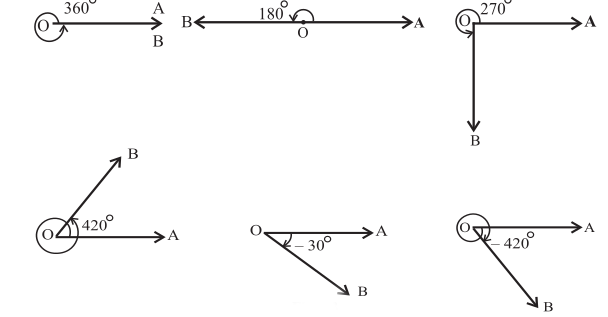
\includegraphics[scale=0.45]{im3.png}
    \end{center}


    \begin{defn}[Radian Measure:]

      Angle subtended at the centre by an arc of length $1$ unit in a
unit circle (circle of radius $1$ unit) is said to have a measure of $1$ radian. In the Fig
$(i)$ and $(ii)$, $OA$ is the initial side and $OB$ is the terminal side. The figures show the
angles whose measures are $1$ radian, $-1$ radian
    \end{defn}
    \begin{center}
      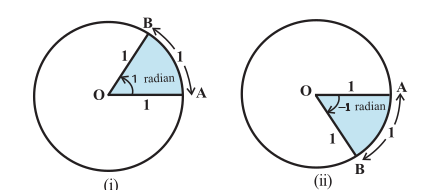
\includegraphics[scale=0.45]{im4.png}
    \end{center}

    Since a circle subtends at the centre
an angle whose radian measure is $2\pi$ and its degree measure is $360°$, it follows that

$2\pi\,radian =360^\circ$ or $\pi \, radian =180^\circ$
\\Then we have
$$1 \, radian =\frac{180^\circ}{\pi}=57^\circ 16'$$
$$1^\circ =\frac{\pi}{180} \,radian=0.01746 \, radian$$

\begin{center}
  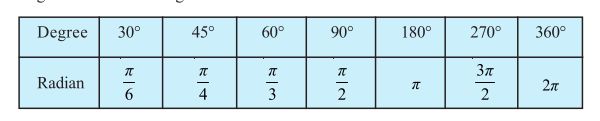
\includegraphics[scale=0.45]{im5.png}
\end{center}
Note that when an angle is expressed in radians, the word 'radian' is frequently omitted.
Thus $\pi= 180^\circ$ and $\frac{\pi}{4}=45^\circ$ are written with the understanding that $\pi$ and $\frac{\pi}{4}$
are radian measures. Thus, we can say that

\begin{center}
  Radian Measure = $\frac{\pi}{180}$ Degree Measure
\end{center}
\begin{center}
  Degree Measure =$\frac{180}{\pi}$ Radian Measure
\end{center}

\begin{subdefn}[Arc, Radius and Angle relation]
  \begin{center}
    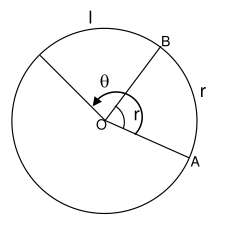
\includegraphics[scale=0.45]{im6.png}
  \end{center}
  Length of the arc of a circle having radius $'r'$
and inclination $'\theta'$ radians is $l=r\theta$.
\end{subdefn}


\begin{defn}[Triganometric Functions:]
  Trigonometric
functions are periodic and thus many natural
phenomena are most readily studies with the
help of trigonometric functions. Unlike
algebraic functions, these functions are not
represented by single letters, instead the
abbreviation sin is used for sine function, cos is
for cosine function, tan is for tangent function,
cosec for cosecant function, sec is for secant
function and cot is for cotangent function. For a
given angle $\theta$, it is usual to write $sin\theta$ for $sin(\theta)$,
etc
  
\end{defn}

\begin{center}
  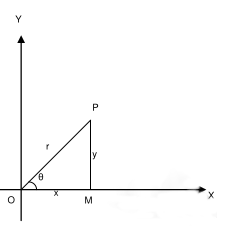
\includegraphics[scale=0.45]{im7.png}
\end{center}

\begin{align*}
sin \theta=\frac{opp\,side}{hypotenuse}=\frac{y}{r}\\
cos \theta=\frac{adjacent\,side}{hypotenuse}=\frac{x}{r}\\
tan \theta=\frac{opp\,side}{adjacent\,side}=\frac{y}{x}\\
cosec \theta = \frac{1}{sin \theta}=\frac{r}{y}\\
sec \theta = \frac{1}{cos \theta}=\frac{r}{x}\\
cot \theta = \frac{1}{tan \theta} = \frac{x}{y}
\end{align*}




  

\begin{subdefn}[Phythagoras' relations]
  \begin{align*}
    sin^2 \theta + cos^2 \theta =1 \\
    sec^2 \theta - tan^2 \theta = 1 \\
    cosec^2 \theta - cot^2 \theta =1
  \end{align*}
  
\end{subdefn}

\begin{subdefn}[Trigonometric Ratios of particular angles]
  \begin{center}
    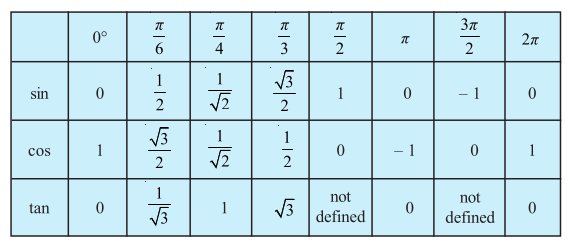
\includegraphics[scale=0.45]{im8.png}
  \end{center}
  
\end{subdefn}

\begin{subdefn}[  Signs of Trigonometric functions in Quadrants]
  \begin{center}
    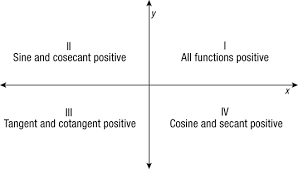
\includegraphics[scale=0.7]{img9.png}
  \end{center}

  \begin{defn}[Domain and range of trigonometric functions]
    \begin{center}
      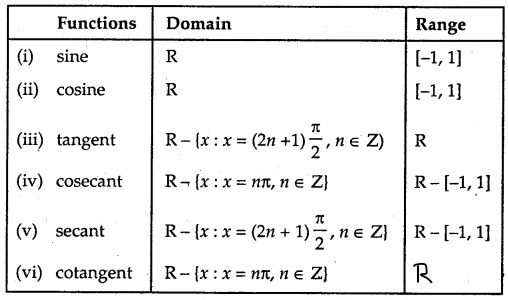
\includegraphics[scale=0.5]{im10.jpg}
    \end{center}
    
  \end{defn}

  \begin{center}
      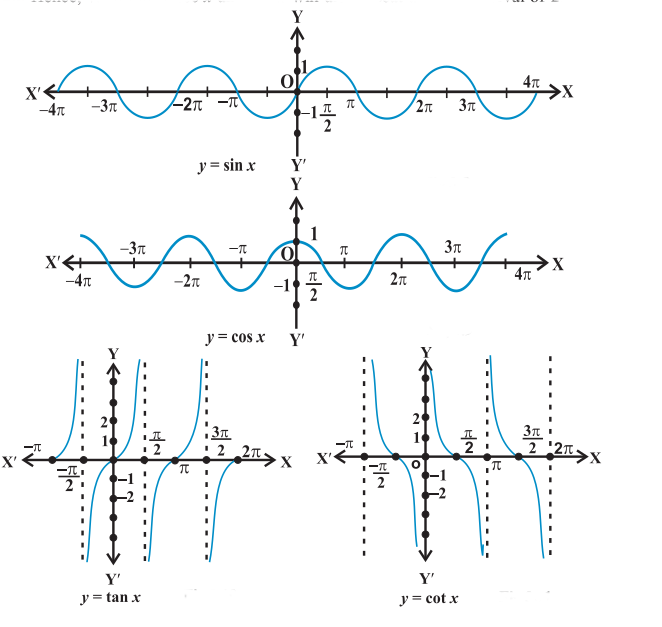
\includegraphics[scale=0.4]{10.png}
      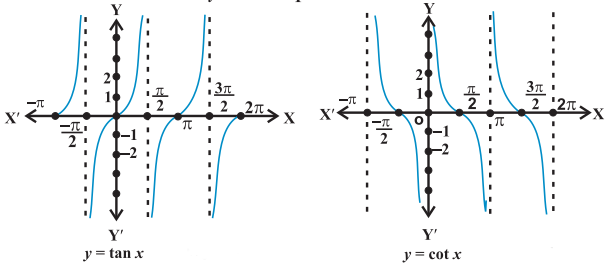
\includegraphics[scale=0.4]{11.png}
      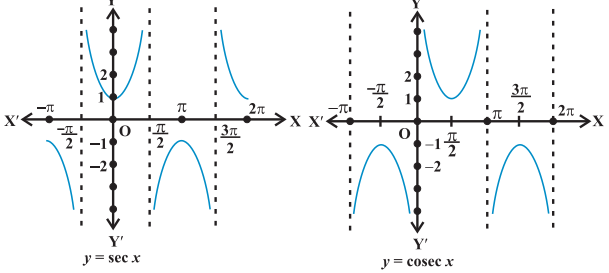
\includegraphics[scale=0.4]{12.png}
  \end{center}
\end{subdefn}
 \subsubsection*{\large \textcolor{red}{Triganometric Functions of larger angles}}
For an angle $\theta$  and integer n\\
\begin{align*}
    sin(n \pi \pm \theta)=sin \theta \\
    cos(n \pi \pm \theta)=cos \theta \\
        tan(n \pi \pm \theta)=tan \theta \\
          cosec(n \pi \pm \theta)=cosec \theta \\
            sec(n \pi \pm \theta)=sec \theta \\
              cot(n \pi \pm \theta)=cot \theta \\
\end{align*}
( even multiple of $90^0 + \theta$)
\begin{align*}
    sin((2n+1) \frac{\pi}{2} \pm \theta)=cos \theta \\
    cos((2n+1) \frac{\pi}{2} \pm \theta)=sin \theta \\
    tan((2n+1) \frac{\pi}{2} \pm \theta)=cot \theta \\
    cot((2n+1) \frac{\pi}{2} \pm \theta)=tan \theta \\
    cosec((2n+1) \frac{\pi}{2} \pm \theta)=sec \theta \\
    sec((2n+1) \frac{\pi}{2} \pm \theta)=cosec \theta \\
\end{align*}
(even multiple of $90^0 + \theta$)
\subsubsection*{\large \textcolor{red}{Compound Angle Formulas}}
\begin{itemize}
    \item $sin(x + y) = sin\, x cos y + cos x \,sin y$

\item $sin(x – y) = sin x \,cos y – cos x\, sin y$

\item $cos(x + y) = cos x\, cos y – sin x \,sin y$

\item $cos(x – y) = cos x\, cos y + sin x\, sin y$

\item  $tan ( x + y) =\frac{tan x + tan y}{1 - tan x\, tan y}$
\item $tan ( x – y) =\frac{tan x – tan y}{1 + tan x\, tan y}$
\item $cot(x+y)=\frac{cotx \,coty-1}{cot x+cot y}$
\item  $cot(x-y)=\frac{cotx \,coty+1}{cot x-cot y}$

\end{itemize}


\subsection*{\large \textcolor{red}{ Multiple Angle Formulas}}
\begin{itemize}
    \item $sin 2x=2 sinx \, cosx=\frac{2tanx}{1+ tan^2 x}$
    \item $sin 3x = 3 sin x – 4 sin^3 x$
    \item $cos 2x =cos^2 x - sin^2 x =1- 2sin^2x=2cos^2x-1=\frac{1-tan^2 x}{1+ tan^2 x}$
    \item  $cos 3x=4 cos^3 x -3 cos x$
    \item $tan 2x =\frac{2 tan /,x }{1- tan^2x}$
    
\end{itemize}

\subsection*{\large \textcolor{red}{Sum Formulas}}

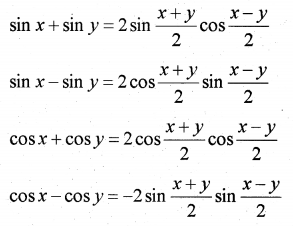
\includegraphics[scale=0.6]{13.png}

\subsection*{\large \textcolor{red}{ Product Formula}}

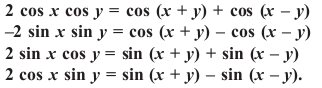
\includegraphics[scale=0.6]{14.png}

\subsubsection*{\large \textcolor{red}{ Solution of Trigonometric Equations}}
sin x = 0 gives $x = n \pi$, where $n \in Z$

cos x = 0 gives $x = (2n + 1)\pi$, where $n \in Z$

tanx = 0 gives $x = n \pi$, where $n \in Z$

sin x = sin y  gives $x = n \pi + (-1)^n y$, where $n \in Z$

cos x = cos y gives $x = 2n\pi ± y$, where $n \in Z$

tan x = tan y gives $x = n\pi + y$, where $n \in Z$
\\
Principal solution is the solution which lies in the interval $0 \leq x \leq 2\pi$.
\end{multicols}

\end{document}


